\chapter{Taking Action \\ (TODO List in Order)}


\section{Canvas}
Now, check the Canvas Teams and see if anything needs updating or changing.
This is the base grounds for all information so make sure that 
that resources, links, competitions are all up to date.

\section{Club Fair Prep}
During the 2nd or 3rd week of September, there will be a club fair for all of the clubs.
This is Math Club's first impression to any outsiders and this is our steady source of new members.
\newline
\newline
You will need:

\begin{itemize}
    \item Candy/Snacks
    \item Poster
    \item Desk [Provided]
    \item Laptop (Activity)
    \item Clipboard + Pens
    \item 10 Lined-Paper
\end{itemize}

\newpage
When interacting with potenial members, mention the key things: tutoring, competitions, awards. \\
If they mention they aren't good at math, offer free tutoring for any topic. \\
If they are more on the math wizard side, offer them the idea of awards like top 10 at State.
\newline
\newline

After the club fair, round up all of the members into a excel sheet seperating them into grade.
\begin{figure}[H]
    \centering
    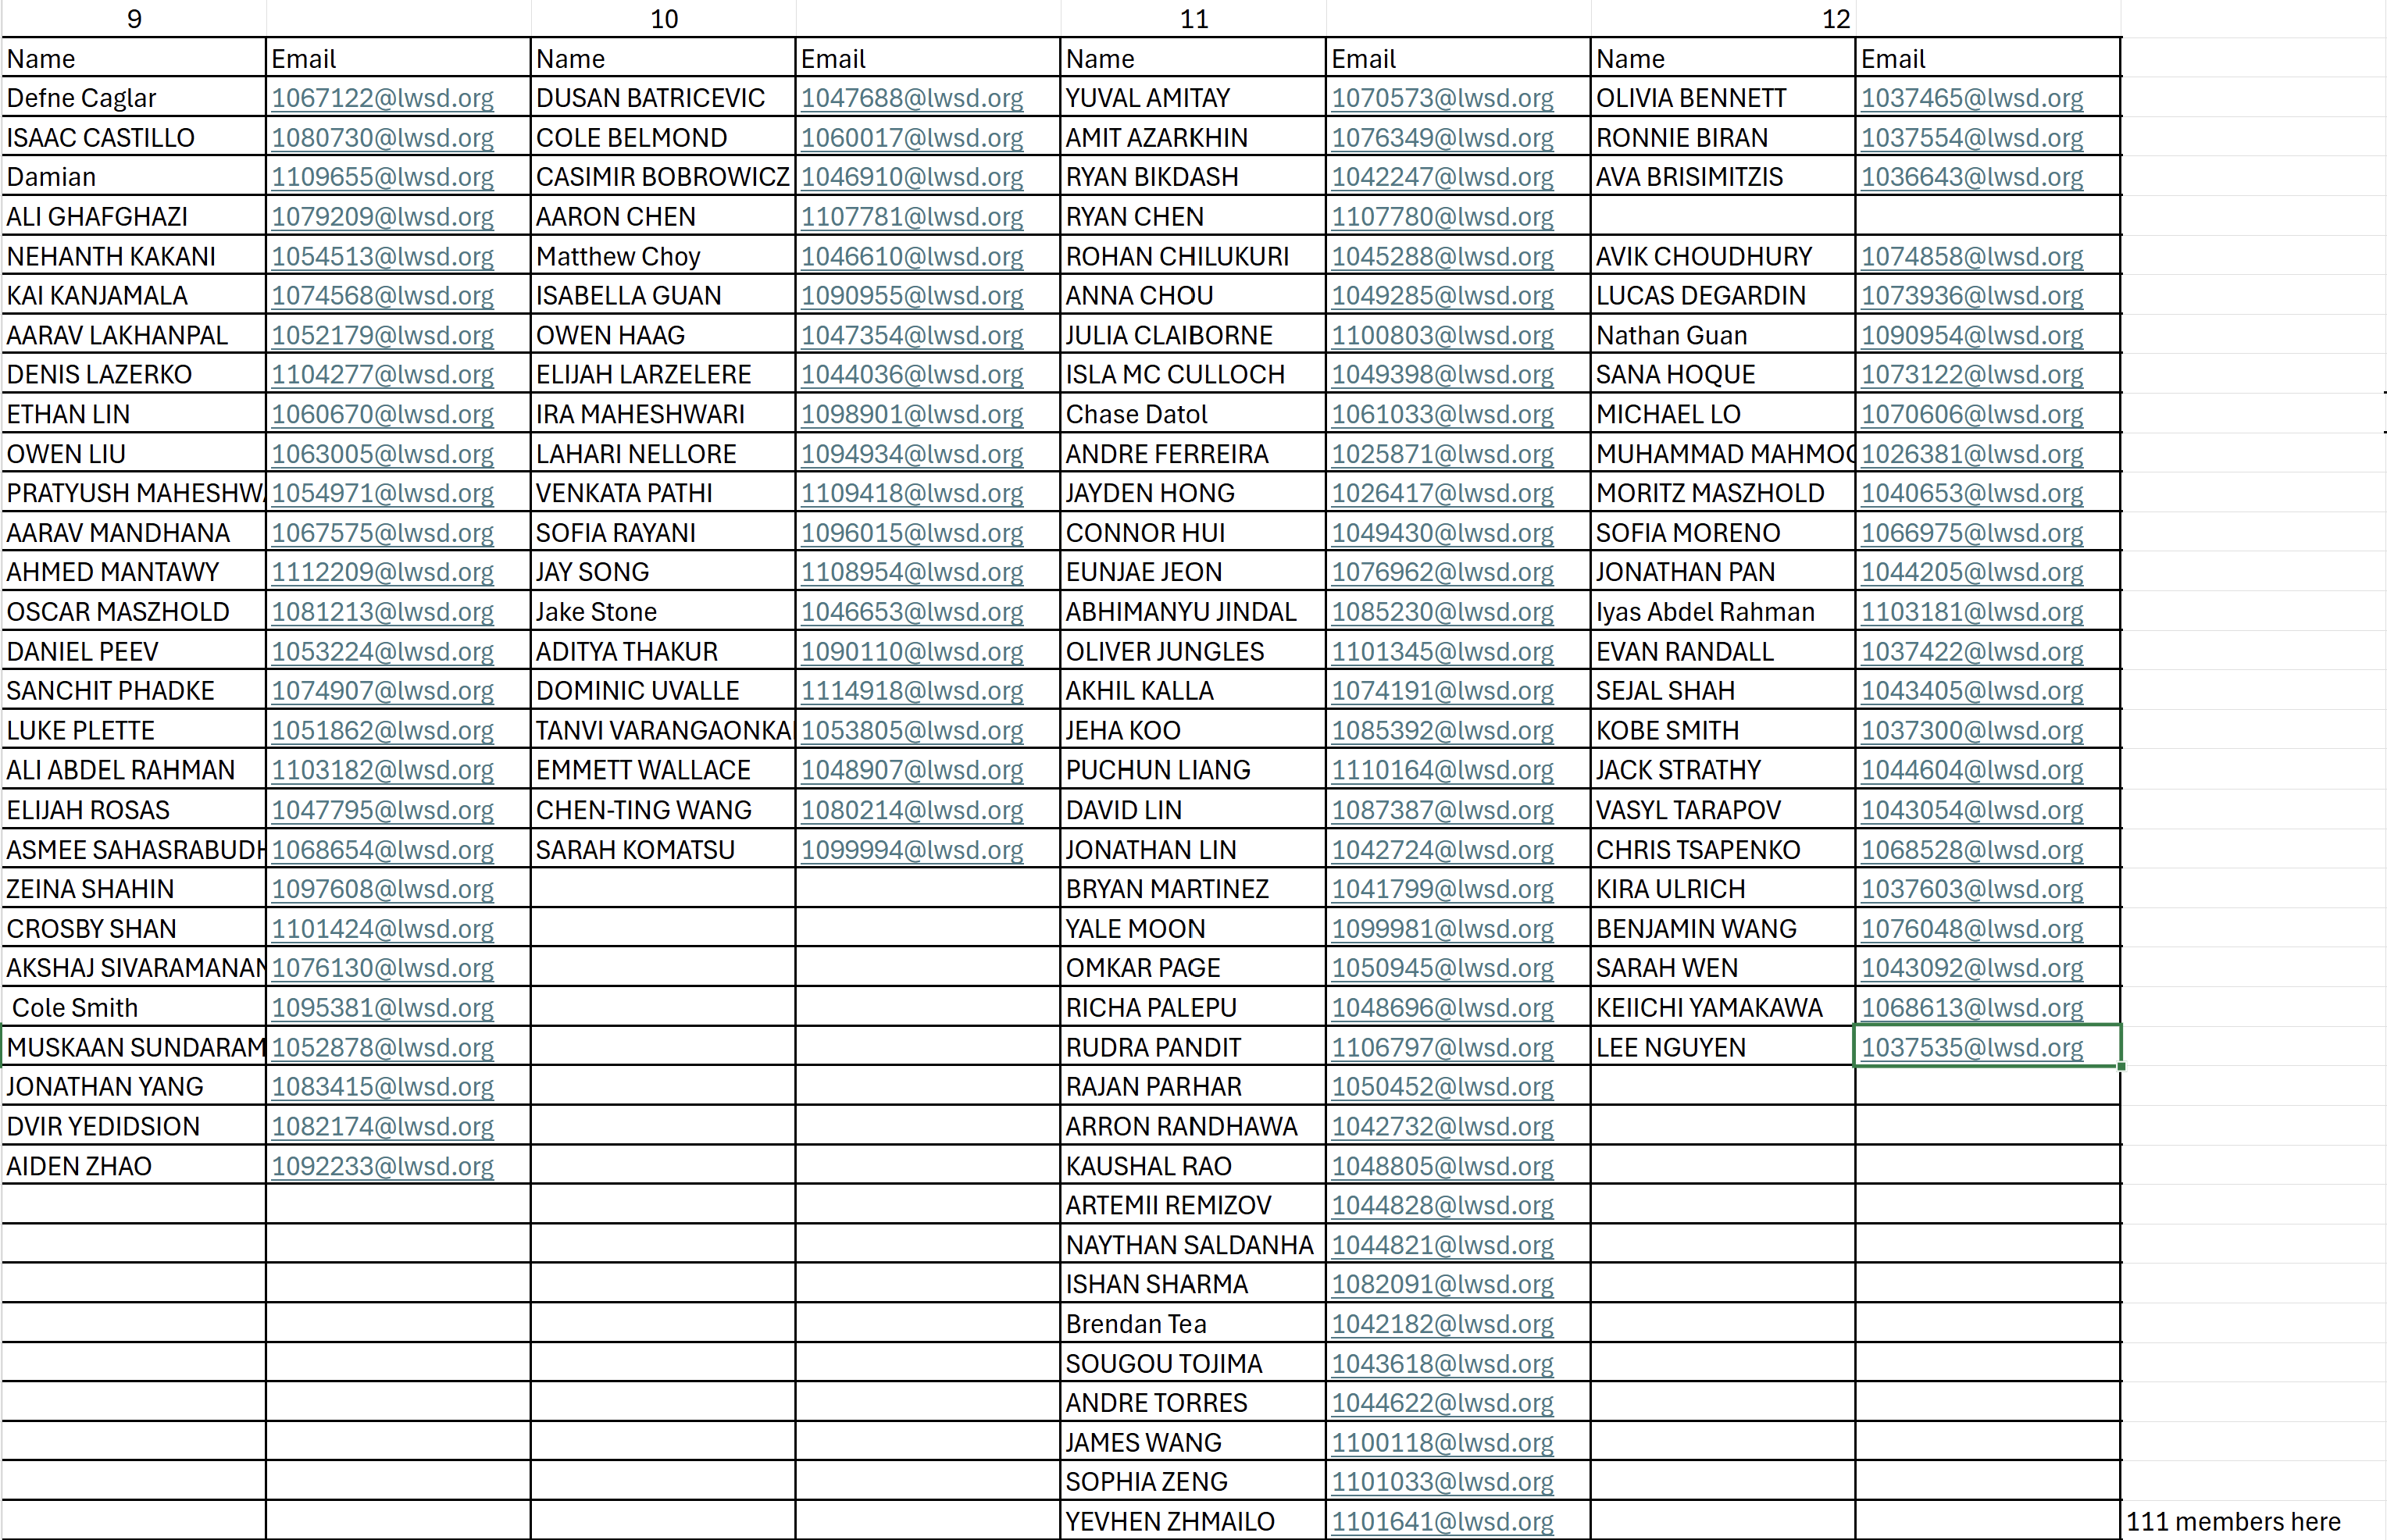
\includegraphics[width=.5\textwidth,height=.5\textheight,keepaspectratio]{members.png}
    \caption{Members list with emails in excel}
    \label{fig:old competition image example}
\end{figure}

In this format, it is easy to copy the emails and transfer them into an email list.
You will then send an email to all of the members. Remember that there is a 100 person limit
when sending emails so you may have to split the email. Send the email to the club officers and
CC the club advisors. Here is a template you may use:

\begin{quote}
Hello, fellow math clubbers,
 
Thank you for your interest in Math Club at today's club fair!

I am excited to announce that we have our \key{first meeting in two weeks on Friday, the 4th of October.} This meeting and all meetings after will be held in Dr. Lu's room, N-272, which is on the second floor of the North Wing.
 
In the first meeting, we will explain what meetings are going to look like, the benefits you reap from attending math club, and introduce some of the fun activities that we have planned for you this year. Throughout the year, we will provide tutoring services, cover various math concepts, and host math competition events as well! 

If you have any questions, feel free to contact me or any of the officers.
We look forward to getting to know all of you and your mathematical aspirations on Friday. Spread the word to all your friends.

Have a great day, \\
Math Club Officers
\end{quote}


\section{Awareness}
    Create flyer posters with QR codes advertising Math Club to put around the school or in math teacher's classes. 
    \key{You will need them ASB approved and permission from teachers.} 
    \begin{figure}[H]
        \centering
        
\includegraphics[width=.5\textwidth,height=.5\textheight,keepaspectratio]{flyer.png}
        \caption{Flyer example | do not scan the QR lmao}
    \end{figure}
    
    
    Additionally, update our club's instagram at \key{$\text{@lwhs\_math}$} with competitions
    and other forms.

\section{Creating PPTs}
You may use past year's ppt as inspiration. \\\\ Here is the general structure:

\begin{enumerate}
    \item Intro Page
    \item When + Where [Friday, Dr. Lu N-272] 
    \item Competitions  
    \item Tutoring \& Volunteer Hours 
    \item Final Take Aways: 
            \begin{itemize}
                \item Fridays N-272  | Can Drop out 
                \item  \# Competitions through the Year 
                \item  Tutoring Volunteer Hours 
                \item  Math Wizard/ academic weapon    
            \end{itemize}
    \item Form [Questions \& Attendance] 
            \begin{itemize}
                \item Name, Email, Grade
                \item AMC 10/12 
                \item Purpose for joining
            \end{itemize}

\end{enumerate}
Some interesting topics this are:

\begin{itemize}
    \item Math Problem Activity
    \item Become a Math Wizard 
    \item Awards/Medals
\end{itemize}

\section{Club Meeting Plans}
This is where you decide what will happen during club meetings.

\noindent
Here is the general structure:
    \begin{enumerate}
        \item Set-Up Math Club [HDMI + Activities]
        \item Wait for people to come 
        \item Start [bang the gong if you want]
        \item Split into Activities
        \item End + Thanks
        \item REPEAT 29x~ Meetings
    \end{enumerate}

\section{Competitions}
    Ms. Martinez will ususally send an email with all of the math competitions for the year. 
    \key{Make sure to inform members 3-4 weeks since permission forms are due 2 weeks before the competition.}

    \begin{figure}[H]
        \centering
        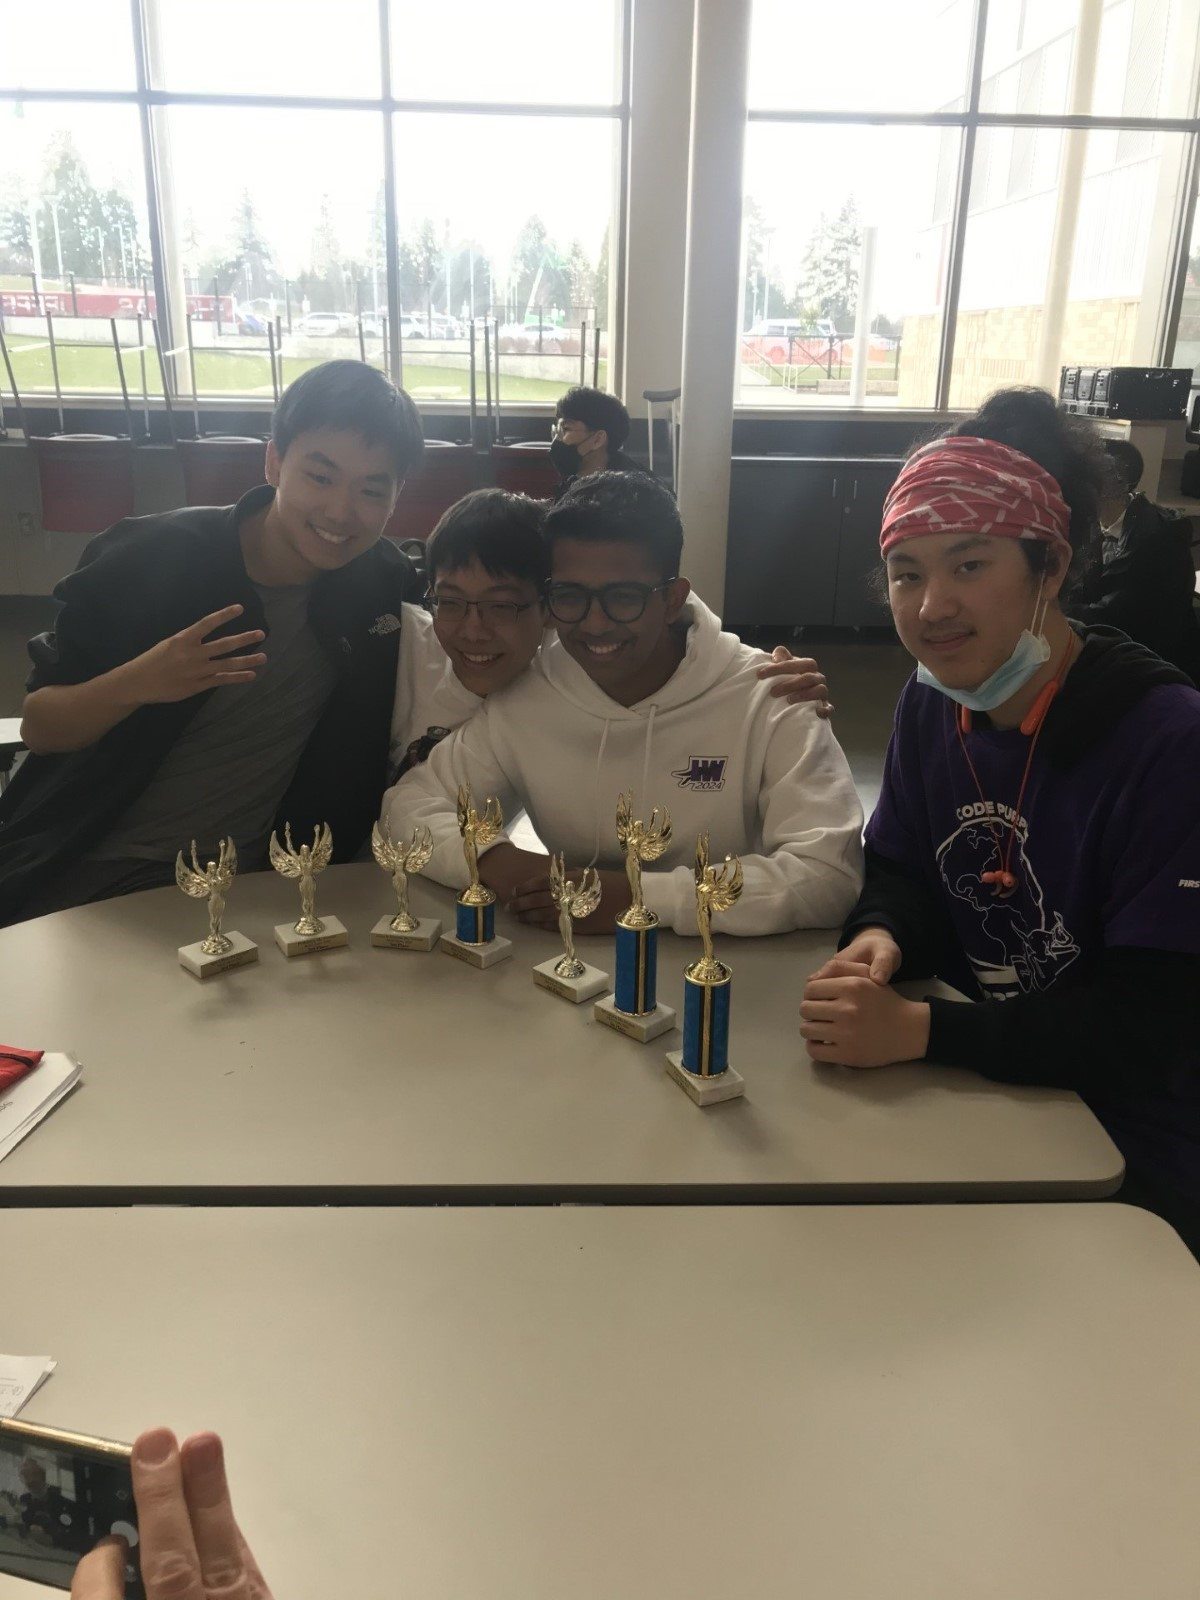
\includegraphics[width=.5\textwidth,height=.5\textheight,keepaspectratio]{example.png}
        \caption{2022-2023 MAO Spring Classic Competition: Logan Chu, Brice Liu, Amish Patra, Bryan H [Left to Right]}
        \label{fig:old competition image example}
    \end{figure}

\section{Fundraising}
After everything, now to acquire funds.
First know which businesses students usually go to and compile a hit-list.
Go to the businesses and ask the manager if they are able to make a fundraising deal.

If that doesen't go well, apply for an ASB Grant by contacting one of the ASB leadership members.
Then, volunteer at concessions for funding also.

\section{Officer Positions}
This wayyyy later on near June. If you have \key{completely finished} the above,
read in the \hyperref[sec:Officer]{ Endgame section} on this. 